
\chapter{\ee\ API}
\label{chap:rest-api}

\section{Introduction}

This chapter provides detailed information about the \ee\ REST API and its target mainly to choreography deployers\footnote{Deployer is the human operator responsible by the deployment process.}.
Understanding the API enables you to write your own code to enact a choreography. 

This chapter is organized as follows. Section \ref{sec:model} presents the data model that defines XML representations exchanged by API messages. Section \ref{sec:api} describes all the operations provided by the REST API, detailing parameters and return structures. Section \ref{sec:client} presents our client implementation that can be used within any Java program.

\section{Data model}
\label{sec:model}

As in any API, \ee\ operations receive and return complex data structures representing real world concepts. 
Figure \ref{img:data_model} presents these concepts in the UML notation.
Although the REST API handles XML representations, we use here the UML notation, since it makes easier to the reader to understand the concepts.

\begin{figure}
\centering
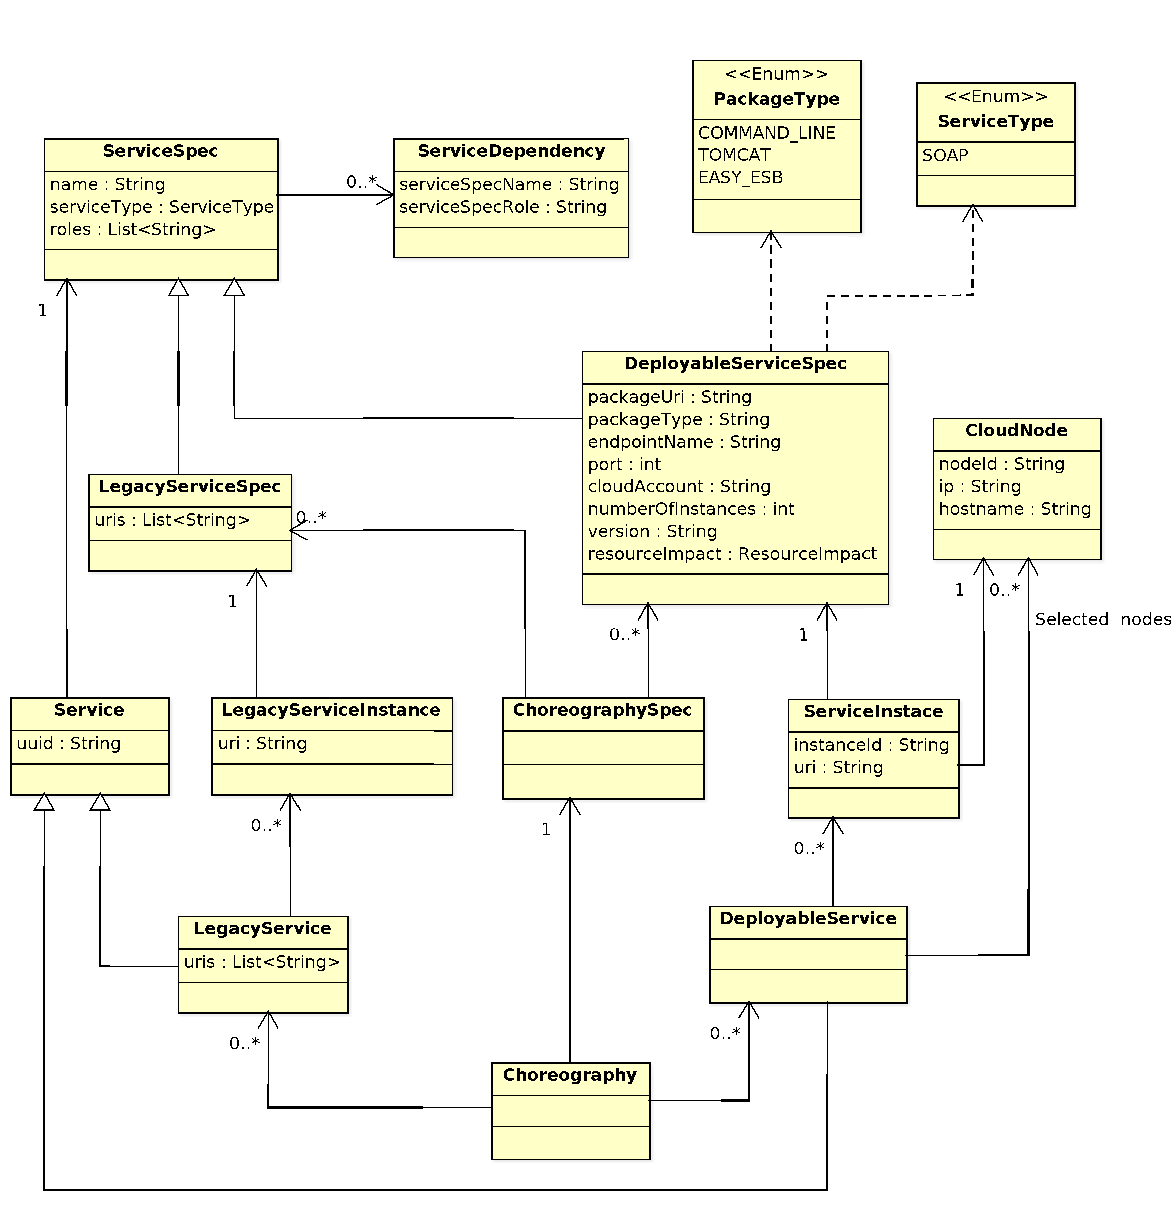
\includegraphics[scale=0.8]{img/data_model.pdf}
\caption{\ee\ REST API data model.}
\label{img:data_model}
\end{figure}

We proceed with a brief explanation about each class:

\begin{description}
\item [ChoreographySpec:] represents what the middleware needs to know to enact a choreography;
\item [ServiceSpec:] a super class for common data of \verb!DeployableServiceSpec! and \verb!LegacyServiceSpec!;
\item [LegacyServiceSpec:] represents an already existing service to used by the choreography;
\item [DeployableServiceSpec:] represents what the middleware needs to know to deploy a service (with one or more instances for load balancing); 
\item [ServiceDependency:] represents dependencies among services (if \verb!service A! invokes \verb!service B!, we say \verb!service A! depends on \verb!service B!);
\item [Choreography:] provides information about a choreography instance;
\item [Service:] a super class for common data of \verb!DeployableService! and \verb!LegacyService!;
\item [LegacyService:] provides information about a legacy service;
\item [DeployableService:] provides information about a deployed service;
\item [ServiceInstance:] provides information about a specific instance, also called replica, of a deployed service (URI, node data etc.). 
\item [LegacyServiceInstance:] provides information about a specific instance of a legacy service. 
\item [Node:] information about the node, including IP address, where a service instance is running.
\end{description}

To request a choreography enactment, it is important to understand very well the \verb!ServiceSpec!, \verb!DeployableServiceSpec!, and the \verb!LegacyServiceSpec! classes. Therefore, the description of them follows:

\begin{enumerate}

\item \verb!ServiceSpec!
	\begin{description}
		\item [name:] a unique character sequence within the choreography specification;
		\item [type:] whether the service is a SOAP service or a REST service. More types can be added as necessary.
		\item [roles:] list of roles implemented by the service;
		\item [dependencies:] list of \verb!ServiceDependency! entries; each entry describes the name of the dependency (matching the \verb!name! attribute), and the the role provided by the dependency;
	\end{description}

\item \verb!DeployableServiceSpec!
	\begin{description}
		\item [packageUri:] the location of the binary file to be deployed;
		\item [packageType:] the type of the deployable package, according to the \verb!PackageType! enumeration\footnote{When the package type i    s COMMAND\_LINE the service will be executed by the ``java -jar'' command.}.
		\item [endpointName:] the endpoint suffix after deployment. For example, if the service will be deployed as \verb!http://<some_ip>/choreos/service!, the endpoint name is \verb!choreos/service!. Note that multiple replicas of a single service will all use the same endpoint;
		\item [port:] the TCP port used by the service. Note that multiple replicas of a single service will all use the same port. Mandatory if type is COMMAND\_LINE;
		\item [owner:] must match a \emph{cloud account} name configured on EE. It will define under which cloud infrastructure the service will be deployed.
		\item [numberOfInstances:] How many instances of the service should be deployed (onto different virtual machines) in order to allow the load to be distributed;
		\item [version:] the service version, which is used by the \ee\ to define which services must be redeployed in a choreography update (not used currently); 
		\item [resourceImpact:] General information regarding the expected type of machine needed to run the service (see \emph{Resource impact specification});
	\end{description}

\item \verb!LegacyServiceSpec!
	\begin{description}
		\item [URIs:] The URIs for the various replicas of the service.
	\end{description}

\end{enumerate}

\subsubsection*{More about dependencies}

In a service composition, some services depends on other services. A service that depends on other services is a \emph{consumer} service, and the service that provides functionality to the dependent service is the \emph{provider}. In simple service compositions, such dependency relations are hardcoded on consumer services. But decoupling the consumer service implementation from the actual provider endpoint is a good practice, which enables dynamic adaptation. Moreover, dependency hardcoding is not possible on cloud environments, since we do not know service addresses before deployment. Therefore, in the CHOReOS environment each consumer service is declared as depending on \emph{roles} rather than other service implementations. The consumer service must receive the actual provider endpoint of a service fulfilling the required role through the \verb!setInvocationAddress! operation, which every consumer service must implement.  

The \ee\ will use \verb!ServiceDependency! data to know which calls it must perform to the  \verb!setInvocationAddress! operation of participant services. Thus, the \ee\ will be able to tell, for example, to \verb!ServiceA! that it must use \verb!ServiceB! as \verb!Role1!, where \verb!ServiceB! is the list of endpoint URIs corresponding to the multiple instances of \verb!ServiceB!. In this way, the CHOReOS middleware provides a \emph{dependency injection}\footnote{Dependency Injection pattern, by Martin Fowler: \url{http://martinfowler.com/articles/injection.html}} mechanism to wire up service dependencies.

\emph{Obs:} to SOAP services, the URI passed to the \texttt{setInvocationAddress} operation does not contain the `\texttt{?wsdl}' suffix.

\subsubsection*{Resource impact specification}

The \verb!DeployableServiceSpec! class has also an attribute to specify non-functional requirements. This attribute is called ``resource impact'', and it can be used by the \verb!NodeSelector! to choose the node in which the service should be deployed. \verb!NodeSelector! will try to choose a node that enables the service to fulfil such requirements.

This attribute is not described in this document because its structure is not fully defined yet. But it is expected to define, among others, required values of CPU, memory, and disk usage.

\subsubsection*{XML representation}

Each class is mapped to and from an XML representation according to the default behaviour of the JAXB API\footnote{Java Architecture for XML Binding (JAXB): allows Java developers to map Java classes to XML representations.}. 
To properly build and read these XML representations, you can rely on the schema definition (Section~ \ref{sec:xsd}). We provide here an example of \verb!ChorSpec! (Listing \ref{lst:chor_spec_xml}) and \verb!Choreography! (Listing \ref{lst:chor_xml}) XML representations to a little choreography with just two services (airline and travel-agency services). 

{\footnotesize
\lstset{language=XML}
\begin{lstlisting}[breaklines, caption=ChorSpec XML representation example., label=lst:chor_spec_xml]
<choreographySpec>
    <deployableServiceSpecs>
        <name>airline</name>
        <roles>airline</roles>
        <serviceType>
            <type>SOAP</type>
        </serviceType>
        <endpointName>airline</endpointName>
        <numberOfInstances>1</numberOfInstances>
        <packageType>
            <type>COMMAND_LINE</type>
        </packageType>
        <packageUri>http://valinhos.ime.usp.br:54080/enact_test/v3/Airline-3.0.0.jar</packageUri>
        <port>1234</port>
        <resourceImpact/>
        <version>0.1</version>
    </deployableServiceSpecs>
    <deployableServiceSpecs>
        <dependencies>
            <serviceSpecName>airline</serviceSpecName>
            <serviceSpecRole>airline</serviceSpecRole>
        </dependencies>
        <name>travelagency</name>
        <roles>travelagency</roles>
        <serviceType>
            <type>SOAP</type>
        </serviceType>
        <endpointName>travelagency</endpointName>
        <numberOfInstances>1</numberOfInstances>
        <packageType>
            <type>COMMAND_LINE</type>
        </packageType>
        <packageUri>http://valinhos.ime.usp.br:54080/enact_test/v3/TravelAgency-3.0.0.jar</packageUri>
        <port>1235</port>
        <resourceImpact/>
        <version>0.1</version>
    </deployableServiceSpecs>
</choreographySpec>
\end{lstlisting}

\begin{lstlisting}[breaklines, caption=Choreography XML representation example., label=lst:chor_xml]
<choreography>
    <choreographySpec>
        <deployableServiceSpecs>
            <name>airline</name>
            <roles>airline</roles>
            <serviceType>
                <type>SOAP</type>
            </serviceType>
            <endpointName>airline</endpointName>
            <numberOfInstances>1</numberOfInstances>
            <packageType>
                <type>COMMAND_LINE</type>
            </packageType>
            <packageUri>http://valinhos.ime.usp.br:54080/enact_test/v3/Airline-3.0.0.jar</packageUri>
            <port>1234</port>
            <resourceImpact/>
            <version>0.1</version>
        </deployableServiceSpecs>
        <deployableServiceSpecs>
            <dependencies>
                <serviceSpecName>airline</serviceSpecName>
                <serviceSpecRole>airline</serviceSpecRole>
            </dependencies>
            <name>travelagency</name>
            <roles>travelagency</roles>
            <serviceType>
                <type>SOAP</type>
            </serviceType>
            <endpointName>travelagency</endpointName>
            <numberOfInstances>1</numberOfInstances>
            <packageType>
                <type>COMMAND_LINE</type>
            </packageType>
            <packageUri>http://valinhos.ime.usp.br:54080/enact_test/v3/TravelAgency-3.0.0.jar</packageUri>
            <port>1235</port>
            <resourceImpact/>
            <version>0.1</version>
        </deployableServiceSpecs>
    </choreographySpec>
    <deployableServices>
        <spec xsi:type="deployableServiceSpec" xmlns:xsi="http://www.w3.org/2001/XMLSchema-instance">
            <dependencies>
                <serviceSpecName>airline</serviceSpecName>
                <serviceSpecRole>airline</serviceSpecRole>
            </dependencies>
            <name>travelagency</name>
            <roles>travelagency</roles>
            <serviceType>
                <type>SOAP</type>
            </serviceType>
            <endpointName>travelagency</endpointName>
            <numberOfInstances>1</numberOfInstances>
            <packageType>
                <type>COMMAND_LINE</type>
            </packageType>
            <packageUri>http://valinhos.ime.usp.br:54080/enact_test/v3/TravelAgency-3.0.0.jar</packageUri>
            <port>1235</port>
            <resourceImpact/>
            <version>0.1</version>
        </spec>
        <UUID>9fb5c93a-b4d1-4a56-9b4b-120e89681e31</UUID>
        <selectedNodes>
            <hostname>choreos-node</hostname>
            <id>2</id>
            <ip>192.168.56.102</ip>
        </selectedNodes>
        <serviceInstances>
            <instanceId>travelagency1</instanceId>
            <nativeUri>http://192.168.56.102:1235/travelagency/</nativeUri>
            <node>
                <hostname>choreos-node</hostname>
                <id>2</id>
                <ip>192.168.56.102</ip>
            </node>
            <serviceSpec>
                <dependencies>
                    <serviceSpecName>airline</serviceSpecName>
                    <serviceSpecRole>airline</serviceSpecRole>
                </dependencies>
                <name>travelagency</name>
                <roles>travelagency</roles>
                <serviceType>
                    <type>SOAP</type>
                </serviceType>
                <endpointName>travelagency</endpointName>
                <numberOfInstances>1</numberOfInstances>
                <packageType>
                    <type>COMMAND_LINE</type>
                </packageType>
                <packageUri>http://valinhos.ime.usp.br:54080/enact_test/v3/TravelAgency-3.0.0.jar</packageUri>
                <port>1235</port>
                <resourceImpact/>
                <version>0.1</version>
            </serviceSpec>
        </serviceInstances>
    </deployableServices>
    <deployableServices>
        <spec xsi:type="deployableServiceSpec" xmlns:xsi="http://www.w3.org/2001/XMLSchema-instance">
            <name>airline</name>
            <roles>airline</roles>
            <serviceType>
                <type>SOAP</type>
            </serviceType>
            <endpointName>airline</endpointName>
            <numberOfInstances>1</numberOfInstances>
            <packageType>
                <type>COMMAND_LINE</type>
            </packageType>
            <packageUri>http://valinhos.ime.usp.br:54080/enact_test/v3/Airline-3.0.0.jar</packageUri>
            <port>1234</port>
            <resourceImpact/>
            <version>0.1</version>
        </spec>
        <UUID>68d8e82b-f6e6-4314-9415-d2a18f61edcf</UUID>
        <selectedNodes>
            <hostname>choreos-node</hostname>
            <id>1</id>
            <ip>192.168.56.101</ip>
        </selectedNodes>
        <serviceInstances>
            <instanceId>airline0</instanceId>
            <nativeUri>http://192.168.56.101:1234/airline/</nativeUri>
            <node>
                <hostname>choreos-node</hostname>
                <id>1</id>
                <ip>192.168.56.101</ip>
            </node>
            <serviceSpec>
                <name>airline</name>
                <roles>airline</roles>
                <serviceType>
                    <type>SOAP</type>
                </serviceType>
                <endpointName>airline</endpointName>
                <numberOfInstances>1</numberOfInstances>
                <packageType>
                    <type>COMMAND_LINE</type>
                </packageType>
                <packageUri>http://valinhos.ime.usp.br:54080/enact_test/v3/Airline-3.0.0.jar</packageUri>
                <port>1234</port>
                <resourceImpact/>
                <version>0.1</version>
            </serviceSpec>
        </serviceInstances>
    </deployableServices>
    <id>1</id>
</choreography>
\end{lstlisting}

}

\section{REST API}
\label{sec:api}

The \ee\ clients access its features through the REST API that is described in this section.

\subsubsection*{Create a choreography}

\begin{tabular}{|c|c|c|c|}
\hline 
\itshape{HTTP Method} & \itshape{URI} & \itshape{Request body} & \itshape{Responses} \\ 
\hline 
POST & /chors & 

\begin{minipage}{2in}
\verb!ChorSpec! XML representation \\ 
(see Listing \ref{lst:chor_spec_xml})
\end{minipage} 
&

\begin{minipage}{2in}
\begin{verbatim}

201 CREATED
location = "/chors/{id}"

400 BAD REQUEST

500 ERROR

\end{verbatim}
\end{minipage} 
\\ 
\hline 
\end{tabular} \\

Creates a specification of the choreography on the \ee.
It does not enact the choreography. 

\emph{Obs:} \texttt{application/xml} is the value to the \texttt{Content Type} header when XML representations are written in the request or response body. 

\subsubsection*{Retrieve choreography information}

\begin{tabular}{|c|c|c|c|}
\hline 
\itshape{HTTP Method} & \itshape{URI} & \itshape{Request body} & \itshape{Responses} \\ 
\hline 
GET & /chors/\{id\} & - &
\begin{minipage}{2in}
\begin{verbatim}

200 OK
location = "/chors/{id}"

Body: 
\end{verbatim}
\verb!Choreography! XML \\
representation \\
(see Listing \ref{lst:chor_xml})
\begin{verbatim}
400 BAD REQUEST

404 NOT FOUND

500 ERROR

\end{verbatim}
\end{minipage} 
\\ 
\hline 
\end{tabular} \\

If this operation is invoked after the creation and before the enactment of a choreography, the body response will be a \verb!Choreography! representation without any deployed service.

\subsubsection*{Enact a choreography}

\begin{tabular}{|c|c|c|c|}
\hline 
\itshape{HTTP Method} & \itshape{URI} & \itshape{Request body} & \itshape{Responses} \\ 
\hline 
POST & /chors/\{id\}/enactment & - &
\begin{minipage}{2in}
\begin{verbatim}

200 OK
location = "/chors/{id}"
Body: 
\end{verbatim}
\verb!Choreography! XML \\
representation \\
(see Listing \ref{lst:chor_xml})
\begin{verbatim}
400 BAD REQUEST

404 NOT FOUND

500 ERROR

\end{verbatim}
\end{minipage} 
\\ 
\hline 
\end{tabular} \\

With this invocation, services will be finally deployed.
The response arrives only after the deployment of all services, if no deployment fails.
It is possible to parse the output to find out failed deployments, which will be the services without associated nodes.

\subsubsection*{Update a choreography (only partially implemented at this time)}

\begin{tabular}{|c|c|c|c|}
\hline 
\itshape{HTTP Method} & \itshape{URI} & \itshape{Request body} & \itshape{Responses} \\ 
\hline 
PUT & /chors/\{id\} & 

\begin{minipage}{2in}
\verb!ChorSpec! XML representation \\ 
(see Listing \ref{lst:chor_spec_xml})
\end{minipage} 
&
\begin{minipage}{2in}
\begin{verbatim}

200 OK
location = "/chors/{id}"
Body: 
\end{verbatim}
\verb!Choreography! XML \\
representation \\
(see Listing \ref{lst:chor_xml})
\begin{verbatim}
400 BAD REQUEST

404 NOT FOUND

500 ERROR

\end{verbatim}
\end{minipage} 
\\ 
\hline 
\end{tabular} \\

This operation has the same behavior of the create choreography operation.
To apply the changes it is necessary to invoke the enactment operation again.
When the new enactment is invoked, the \ee\ will detect the changes that have
been inserted in the choreography and deploys new services, remove unneeded services and redeploy
services where some aspect (such as version number, number of instances etc) has changed.
Currently, the only detected changes are increased or decreased number of instances
and increased or decreased memory consumption. Services on the old and new versions
of the choreography are correlated by means of the \texttt{name} attribute of ServiceSpec.

\section{Java client}
\label{sec:client}

In the \verb!EnactmentEngineAPI! project there is the \verb!EEClient! class, which implements the \verb!EnactmentEngine! interface (Listing \ref{lst:java_interface}) and handles the REST communication with the Enactment Engine server. This means you can invoke the \ee by using a simple Java object, without worrying with XML details.

{\footnotesize
\lstset{language=Java}
\begin{lstlisting}[caption=\ee\ Java interface., label=lst:java_interface]
package org.ow2.choreos.chors;

import org.ow2.choreos.chors.datamodel.Choreography;
import org.ow2.choreos.chors.datamodel.ChoreographySpec;

public interface EnactmentEngine {

    public String createChoreography(ChoreographySpec chor);

    public Choreography getChoreography(String chorId) 
        throws ChoreographyNotFoundException;

    public Choreography enactChoreography(String chorId) 
        throws EnactmentException, ChoreographyNotFoundException;

    public void updateChoreography(String chorId, ChoreographySpec spec) 
        throws EnactmentException, ChoreographyNotFoundException;

}
\end{lstlisting}
}

To use the \ee\ Java client in your code, it's enough to import the API project into your project. One way of doing this is using Maven: install the API project into your local maven repo (\texttt{EnactmentEngineAPI\$mvn install}), add it as a dependency of your project by editing your pom.xml (Listing~\ref{lst:ee_api_maven}), and finally compile your project.

{\footnotesize
\lstset{language=XML}
\begin{lstlisting}[caption=Adding EnactmentEngineAPI as a dependency of your project., label=lst:ee_api_maven]
<dependency>
  <groupId>org.ow2.choreos</groupId>
  <artifactId>EnactmentEngineAPI</artifactId>
  <version>0.0.1-SNAPSHOT</version>
</dependency>
\end{lstlisting}
}

The Listing~\ref{lst:chor_spec_example_java} shows an example of how to use the Java API to create a choreography specification. This example is equivalent to the XML in Listing~\ref{lst:chor_spec_xml}.

{\footnotesize
\lstset{language=Java}
\begin{lstlisting}[caption=Example of choreography specification using the Java API., label=lst:chor_spec_example_java]
public class ChorSpecExample {

    public static final String AIRLINE = "airline";
    public static final String TRAVEL_AGENCY = "travelagency";
    public static final String AIRLINE_JAR = 
            "http://valinhos.ime.usp.br:54080/airline.jar";
    public static final String TRAVEL_AGENCY_JAR = 
            "http://valinhos.ime.usp.br:54080/travel.jar";
    public static final int AIRLINE_PORT = 1234;
    public static final int TRAVEL_AGENCY_PORT = 1235;

    private ChoreographySpec chorSpec;
    private DeployableServiceSpec airlineSpec;
    private DeployableServiceSpec travelSpec;

    public ChoreographySpec getChorSpec() {
        createAirlineSpec();
        createTravelAgencySpec();
        chorSpec = new ChoreographySpec(this.airlineSpec, this.travelSpec);
        return chorSpec;
    }

    private void createAirlineSpec() {
        airlineSpec = new DeployableServiceSpec();
        airlineSpec.setName(AIRLINE);
        airlineSpec.setServiceType(ServiceType.SOAP);
        airlineSpec.setPackageType(PackageType.COMMAND_LINE);
        airlineSpec.setPackageUri(AIRLINE_JAR);
        airlineSpec.setPort(AIRLINE_PORT);
        airlineSpec.setEndpointName(AIRLINE);
        airlineSpec.setRoles(Collections.singletonList(AIRLINE));
    }

    private void createTravelAgencySpec() {
        travelSpec = new DeployableServiceSpec();
        travelSpec.setName(TRAVEL_AGENCY);
        travelSpec.setServiceType(ServiceType.SOAP);
        travelSpec.setPackageType(PackageType.COMMAND_LINE);
        travelSpec.setPackageUri(TRAVEL_AGENCY_JAR);
        travelSpec.setPort(TRAVEL_AGENCY_PORT);
        travelSpec.setEndpointName(TRAVEL_AGENCY);
        travelSpec.setRoles(Collections.singletonList(TRAVEL_AGENCY));
        ServiceDependency dependency = new ServiceDependency();
        dependency.setServiceSpecName(AIRLINE);
        dependency.setServiceSpecRole(AIRLINE);
        travelSpec.addDependency(dependency);
    }
\end{lstlisting}
}

Finally, Listing~\ref{lst:java_chor_enactment} is an example of how to use the Java API to invoke the EE.

{\footnotesize
\begin{lstlisting}[breaklines, caption={Deploying a choreography using the Java API.}, label={lst:java_chor_enactment}]
public class Enactment {

    public static void main(String[] args) throws EnactmentException, ChoreographyNotFoundException {

        final String EE_URI = "http://localhost:9102/enactmentengine";
        EnactmentEngine ee = new EnactmentEngineClient(EE_URI);
        ChorSpecExample example = new ChorSpecExample();
        ChoreographySpec chorSpec = example.getChorSpec();

        String chorId = ee.createChoreography(chorSpec);
        Choreography chor = ee.enactChoreography(chorId);

        System.out.println(chor); // checking output
    }
}
\end{lstlisting}
}

\section{Choreography XML Schema Definition (XSD file)}
\label{sec:xsd}

{\footnotesize

\lstset{language=XML}

\begin{lstlisting}[caption=, label=lst:chor_xsd, breaklines]
ChorSpec XSD:
<?xml version="1.0" encoding="UTF-8"?><xs:schema xmlns:xs="http://www.w3.org/2001/XMLSchema" version="1.0">
<xs:element name="choreographySpec" type="choreographySpec"/>
<xs:element name="deployableServiceSpec" type="deployableServiceSpec"/>
<xs:element name="legacyServiceSpec" type="legacyServiceSpec"/>
<xs:element name="resourceImpact" type="resourceImpact"/>
<xs:complexType name="choreographySpec">
        <xs:sequence>
            <xs:element maxOccurs="unbounded" minOccurs="0" name="deployableServiceSpecs" nillable="true" type="deployableServiceSpec"/>
            <xs:element maxOccurs="unbounded" minOccurs="0" name="legacyServiceSpecs" nillable="true" type="legacyServiceSpec"/>
        </xs:sequence>
    </xs:complexType>
<xs:complexType name="deployableServiceSpec">
        <xs:complexContent>
            <xs:extension base="serviceSpec">
                <xs:sequence>
                    <xs:element minOccurs="0" name="cloudAccount" type="xs:string"/>
                    <xs:element minOccurs="0" name="desiredQoS" type="desiredQoS"/>
                    <xs:element minOccurs="0" name="endpointName" type="xs:string"/>
                    <xs:element name="numberOfInstances" type="xs:int"/>
                    <xs:element minOccurs="0" name="packageType" type="packageType"/>
                    <xs:element minOccurs="0" name="packageUri" type="xs:string"/>
                    <xs:element name="port" type="xs:int"/>
                    <xs:element minOccurs="0" ref="resourceImpact"/>
                    <xs:element minOccurs="0" name="version" type="xs:string"/>
                </xs:sequence>
            </xs:extension>
        </xs:complexContent>
    </xs:complexType>
<xs:complexType abstract="true" name="serviceSpec">
        <xs:sequence>
            <xs:element maxOccurs="unbounded" minOccurs="0" name="dependencies" nillable="true" type="serviceDependency"/>
            <xs:element minOccurs="0" name="name" type="xs:string"/>
            <xs:element maxOccurs="unbounded" minOccurs="0" name="roles" nillable="true" type="xs:string"/>
            <xs:element minOccurs="0" name="serviceType" type="serviceType"/>
        </xs:sequence>
    </xs:complexType>
<xs:complexType name="desiredQoS">
        <xs:sequence>
            <xs:element minOccurs="0" name="responseTimeMetric" type="responseTimeMetric"/>
        </xs:sequence>
    </xs:complexType>
<xs:complexType name="responseTimeMetric">
        <xs:sequence>
            <xs:element name="acceptablePercentage" type="xs:float"/>
            <xs:element name="maxDesiredResponseTime" type="xs:float"/>
        </xs:sequence>
    </xs:complexType>
<xs:complexType name="packageType">
        <xs:sequence>
            <xs:element minOccurs="0" name="type" type="xs:string"/>
        </xs:sequence>
    </xs:complexType>
<xs:complexType name="resourceImpact">
        <xs:sequence>
            <xs:element minOccurs="0" name="memory" type="memoryType"/>
            <xs:element minOccurs="0" name="cpu" type="xs:string"/>
            <xs:element minOccurs="0" name="storage" type="xs:string"/>
            <xs:element minOccurs="0" name="network" type="xs:string"/>
        </xs:sequence>
    </xs:complexType>
<xs:complexType name="serviceDependency">
        <xs:sequence>
            <xs:element minOccurs="0" name="serviceSpecName" type="xs:string"/>
            <xs:element minOccurs="0" name="serviceSpecRole" type="xs:string"/>
        </xs:sequence>
    </xs:complexType>
<xs:complexType name="serviceType">
        <xs:sequence>
            <xs:element minOccurs="0" name="type" type="xs:string"/>
        </xs:sequence>
    </xs:complexType>
<xs:complexType name="legacyServiceSpec">
        <xs:complexContent>
            <xs:extension base="serviceSpec">
                <xs:sequence>
                    <xs:element maxOccurs="unbounded" minOccurs="0" name="nativeURIs" nillable="true" type="xs:string"/>
                </xs:sequence>
            </xs:extension>
        </xs:complexContent>
    </xs:complexType>
<xs:simpleType name="memoryType">
        <xs:restriction base="xs:string">
            <xs:enumeration value="SMALL"/>
            <xs:enumeration value="MEDIUM"/>
            <xs:enumeration value="LARGE"/>
        </xs:restriction>
    </xs:simpleType>
</xs:schema>

Choreography XSD:
<?xml version="1.0" encoding="UTF-8"?><xs:schema xmlns:xs="http://www.w3.org/2001/XMLSchema" version="1.0">
<xs:element name="choreography" type="choreography"/>
<xs:element name="choreographySpec" type="choreographySpec"/>
<xs:element name="cloudNode" type="cloudNode"/>
<xs:element name="deployableService" type="deployableService"/>
<xs:element name="deployableServiceSpec" type="deployableServiceSpec"/>
<xs:element name="legacyServiceSpec" type="legacyServiceSpec"/>
<xs:element name="resourceImpact" type="resourceImpact"/>
<xs:complexType name="choreography">
        <xs:sequence>
            <xs:element minOccurs="0" ref="choreographySpec"/>
            <xs:element maxOccurs="unbounded" minOccurs="0" name="deployableServices" nillable="true" type="deployableService"/>
            <xs:element minOccurs="0" name="id" type="xs:string"/>
            <xs:element maxOccurs="unbounded" minOccurs="0" name="legacyServices" nillable="true" type="legacyService"/>
        </xs:sequence>
    </xs:complexType>
<xs:complexType name="choreographySpec">
        <xs:sequence>
            <xs:element maxOccurs="unbounded" minOccurs="0" name="deployableServiceSpecs" nillable="true" type="deployableServiceSpec"/>
            <xs:element maxOccurs="unbounded" minOccurs="0" name="legacyServiceSpecs" nillable="true" type="legacyServiceSpec"/>
        </xs:sequence>
    </xs:complexType>
<xs:complexType name="deployableServiceSpec">
        <xs:complexContent>
            <xs:extension base="serviceSpec">
                <xs:sequence>
                    <xs:element minOccurs="0" name="cloudAccount" type="xs:string"/>
                    <xs:element minOccurs="0" name="desiredQoS" type="desiredQoS"/>
                    <xs:element minOccurs="0" name="endpointName" type="xs:string"/>
                    <xs:element name="numberOfInstances" type="xs:int"/>
                    <xs:element minOccurs="0" name="packageType" type="packageType"/>
                    <xs:element minOccurs="0" name="packageUri" type="xs:string"/>
                    <xs:element name="port" type="xs:int"/>
                    <xs:element minOccurs="0" ref="resourceImpact"/>
                    <xs:element minOccurs="0" name="version" type="xs:string"/>
                </xs:sequence>
            </xs:extension>
        </xs:complexContent>
    </xs:complexType>
<xs:complexType abstract="true" name="serviceSpec">
        <xs:sequence>
            <xs:element maxOccurs="unbounded" minOccurs="0" name="dependencies" nillable="true" type="serviceDependency"/>
            <xs:element minOccurs="0" name="name" type="xs:string"/>
            <xs:element maxOccurs="unbounded" minOccurs="0" name="roles" nillable="true" type="xs:string"/>
            <xs:element minOccurs="0" name="serviceType" type="serviceType"/>
        </xs:sequence>
    </xs:complexType>
<xs:complexType name="desiredQoS">
        <xs:sequence>
            <xs:element minOccurs="0" name="responseTimeMetric" type="responseTimeMetric"/>
        </xs:sequence>
    </xs:complexType>
<xs:complexType name="responseTimeMetric">
        <xs:sequence>
            <xs:element name="acceptablePercentage" type="xs:float"/>
            <xs:element name="maxDesiredResponseTime" type="xs:float"/>
        </xs:sequence>
    </xs:complexType>
<xs:complexType name="packageType">
        <xs:sequence>
            <xs:element minOccurs="0" name="type" type="xs:string"/>
        </xs:sequence>
    </xs:complexType>
<xs:complexType name="resourceImpact">
        <xs:sequence>
            <xs:element minOccurs="0" name="memory" type="memoryType"/>
            <xs:element minOccurs="0" name="cpu" type="xs:string"/>
            <xs:element minOccurs="0" name="storage" type="xs:string"/>
            <xs:element minOccurs="0" name="network" type="xs:string"/>
        </xs:sequence>
    </xs:complexType>
<xs:complexType name="serviceDependency">
        <xs:sequence>
            <xs:element minOccurs="0" name="serviceSpecName" type="xs:string"/>
            <xs:element minOccurs="0" name="serviceSpecRole" type="xs:string"/>
        </xs:sequence>
    </xs:complexType>
<xs:complexType name="serviceType">
        <xs:sequence>
            <xs:element minOccurs="0" name="type" type="xs:string"/>
        </xs:sequence>
    </xs:complexType>
<xs:complexType name="legacyServiceSpec">
        <xs:complexContent>
            <xs:extension base="serviceSpec">
                <xs:sequence>
                    <xs:element maxOccurs="unbounded" minOccurs="0" name="nativeURIs" nillable="true" type="xs:string"/>
                </xs:sequence>
            </xs:extension>
        </xs:complexContent>
    </xs:complexType>
<xs:complexType name="deployableService">
        <xs:complexContent>
            <xs:extension base="service">
                <xs:sequence>
                    <xs:element maxOccurs="unbounded" minOccurs="0" name="selectedNodes" nillable="true" type="cloudNode"/>
                    <xs:element maxOccurs="unbounded" minOccurs="0" name="serviceInstances" nillable="true" type="serviceInstance"/>
                </xs:sequence>
            </xs:extension>
        </xs:complexContent>
    </xs:complexType>
<xs:complexType abstract="true" name="service">
        <xs:sequence>
            <xs:element minOccurs="0" name="spec" type="serviceSpec"/>
            <xs:element minOccurs="0" name="UUID" type="xs:string"/>
        </xs:sequence>
    </xs:complexType>
<xs:complexType name="cloudNode">
        <xs:sequence>
            <xs:element minOccurs="0" name="cpus" type="xs:int"/>
            <xs:element minOccurs="0" name="hostname" type="xs:string"/>
            <xs:element minOccurs="0" name="id" type="xs:string"/>
            <xs:element minOccurs="0" name="image" type="xs:string"/>
            <xs:element minOccurs="0" name="ip" type="xs:string"/>
            <xs:element minOccurs="0" name="privateKeyFile" type="xs:string"/>
            <xs:element minOccurs="0" name="ram" type="xs:int"/>
            <xs:element minOccurs="0" name="so" type="xs:string"/>
            <xs:element minOccurs="0" name="state" type="xs:int"/>
            <xs:element minOccurs="0" name="storage" type="xs:int"/>
            <xs:element minOccurs="0" name="user" type="xs:string"/>
            <xs:element minOccurs="0" name="zone" type="xs:string"/>
        </xs:sequence>
    </xs:complexType>
<xs:complexType name="serviceInstance">
        <xs:sequence>
            <xs:element minOccurs="0" name="instanceId" type="xs:string"/>
            <xs:element minOccurs="0" name="nativeUri" type="xs:string"/>
            <xs:element minOccurs="0" name="node" type="cloudNode"/>
            <xs:element minOccurs="0" name="serviceSpec" type="deployableServiceSpec"/>
        </xs:sequence>
    </xs:complexType>
<xs:complexType name="legacyService">
        <xs:complexContent>
            <xs:extension base="service">
                <xs:sequence>
                    <xs:element maxOccurs="unbounded" minOccurs="0" name="legacyServiceInstances" nillable="true" type="legacyServiceInstance"/>
                </xs:sequence>
            </xs:extension>
        </xs:complexContent>
    </xs:complexType>
<xs:complexType name="legacyServiceInstance">
        <xs:sequence>
            <xs:element minOccurs="0" name="spec" type="legacyServiceSpec"/>
            <xs:element minOccurs="0" name="uri" type="xs:string"/>
        </xs:sequence>
    </xs:complexType>
<xs:simpleType name="memoryType">
        <xs:restriction base="xs:string">
            <xs:enumeration value="SMALL"/>
            <xs:enumeration value="MEDIUM"/>
            <xs:enumeration value="LARGE"/>
        </xs:restriction>
    </xs:simpleType>
</xs:schema>
\end{lstlisting}
}
